\documentclass{beamer}
\usepackage{graphicx}
\usepackage{xcolor}
\usepackage{tikz}

\mode<presentation>

%\newif\ifbeamer@secheader
%\beamer@secheaderfalse

%\DeclareOptionBeamer{secheader}{\beamer@secheadertrue}
\ProcessOptionsBeamer

\setbeamertemplate{navigation symbols}{} % Removes navigation buttons


\useoutertheme[footline=authorinstitutetitle,subsection=false]{smoothbars}
\makeatletter
% Custom footline setup
\newcommand{\frameofframes}{/}
\newcommand{\setframeofframes}[1]{\renewcommand{\frameofframes}{#1}}

\setbeamertemplate{footline} 
{%
    \begin{beamercolorbox}[colsep=1.5pt]{upper separation line foot}
    \end{beamercolorbox}
    \begin{beamercolorbox}[ht=2.5ex,dp=1.125ex,%
      leftskip=.3cm,rightskip=.3cm plus1fil]{author in head/foot}%
      \leavevmode{\usebeamerfont{author in head/foot}\insertshortauthor}%
      \hfill%
      {\usebeamerfont{institute in head/foot}\usebeamercolor[fg]{institute in head/foot}\insertshortinstitute}%
    \end{beamercolorbox}%
    \begin{beamercolorbox}[ht=2.5ex,dp=1.125ex,%
      leftskip=.3cm,rightskip=.3cm plus1fil]{title in head/foot}%
      {\usebeamerfont{title in head/foot}\insertshorttitle}%
      \hfill%
      {\usebeamerfont{frame number}\usebeamercolor[fg]{frame number}\insertframenumber~\frameofframes~\inserttotalframenumber}
    \end{beamercolorbox}%
    \begin{beamercolorbox}[colsep=1.5pt]{lower separation line foot}
    \end{beamercolorbox}
    %\hfill 
\includegraphics[width=0.1\linewidth]{logo.jpg} % Add this line to include the logo
}
\makeatother

% Theme settings
\useinnertheme{circles}

% Color customizations
\xdefinecolor{shisu}{rgb}{0,0.384,0.675}  % RGB #82318E
\setbeamercolor{footline}{bg=shisu}
\setbeamercolor{frametitle}{bg=shisu,fg=white}
\setbeamercolor{title}{bg=shisu}
\setbeamerfont{frametitle}{size=\large}

% Bibliography and caption settings
\setbeamertemplate{bibliography item}[text]
\setbeamertemplate{caption}[numbered]

% Color palettes
\setbeamercolor{palette primary}{use=structure,fg=white,bg=structure.fg}
\setbeamercolor{palette secondary}{use=structure,fg=white,bg=structure.fg!75!black}
\setbeamercolor{palette tertiary}{use=structure,fg=white,bg=structure.fg!50!black}
\setbeamercolor{palette quaternary}{fg=white,bg=structure.fg!50!black}
\setbeamercolor{titlelike}{parent=palette primary}

% Block and sidebar colors
\setbeamercolor{block title}{bg=shisu,fg=white}
\setbeamercolor*{block title example}{use={normal text,example text},bg=white,fg=shisu}
\setbeamercolor{item projected}{fg=white}
\setbeamercolor{sidebar}{bg=shisu}
\setbeamercolor{structure}{fg=shisu}

% Section and subsection styling
\setbeamercolor{section in sidebar}{fg=brown}
\setbeamercolor{subsection in sidebar}{fg=brown}

%\iffalse
% Table of contents at the start of sections/subsections
\AtBeginSection[]{
	\begin{frame}
		\tableofcontents[sectionstyle=show/shaded,subsectionstyle=show/shaded/hide,subsubsectionstyle=show/shaded/hide]
	\end{frame}
}
\AtBeginSubsection[]{
	\begin{frame}
		\tableofcontents[sectionstyle=show/shaded,subsectionstyle=show/shaded/hide,subsubsectionstyle=show/shaded/hide]
	\end{frame}
} 
%\fi

% Add logo overlay in the bottom-right corner
\addtobeamertemplate{background}{%
    \begin{tikzpicture}[remember picture,overlay]
        \node[anchor=south east,xshift= 4pt,yshift=15pt] at (current page.south east) {
\includegraphics[width=0.1\linewidth]{logo.jpg}};
    \end{tikzpicture}
}


% Title Information
\title{Clustering Algorithms: k-Means and k-Medoids}
\author{Gandholi Sarat}
\institute{Sri Sathya Sai Institute of Higher Learning}
\date{\today}

\begin{document}

% Title Page
\begin{frame}
    \titlepage
\end{frame}

\section{k-Means}
\begin{frame}{k-Means}
    \begin{itemize}
        \item k-Means is a widely used clustering algorithm due to its efficiency.
        \item Time complexity: \(O(Nmq)\), where \(q\) is the number of iterations, and m is number of clusters.
        \item Suitable for large datasets.
    \end{itemize}
    \begin{figure}
        \centering
        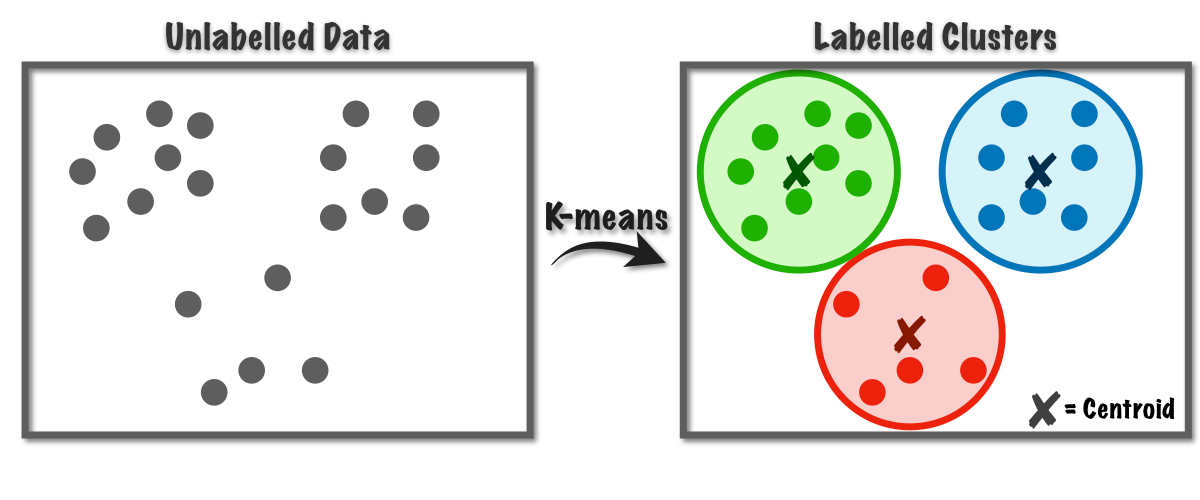
\includegraphics[width=0.8\linewidth]{1.png}
    \end{figure}
\end{frame}


% Section: Advantages and Drawbacks
\section{Advantages and Drawbacks}
\begin{frame}{Advantages of k-Means}
    \begin{itemize}
        \item Fast and computationally efficient.
        \item Simple to implement and interpret.
        \item Can be extended for different clustering problems.
    \end{itemize}
\end{frame}

\begin{frame}{Drawbacks of k-Means}
    \begin{itemize}
        \item Sensitive to outliers and noise.
        \item Struggles with non-spherical clusters.
        \item Generally applicable to data sets with continuous valued feature vectors
    \end{itemize}
\end{frame}

% Section: k-Medoids Algorithm
\section{k-Medoids}
\begin{frame}{Introduction to k-Medoids}
    \begin{itemize}
        \item  In the k-medoids methods,each cluster is represented by a vector selected among the elements of X, and we will refer to it as the \textbf{medoid}
        \item More robust to \textbf{outliers}.
        \item Works for both continuous and discrete datasets.
    \end{itemize}
\end{frame}
\begin{frame}{K-mean Vs K-Medoids}
    \begin{figure}
        \centering
        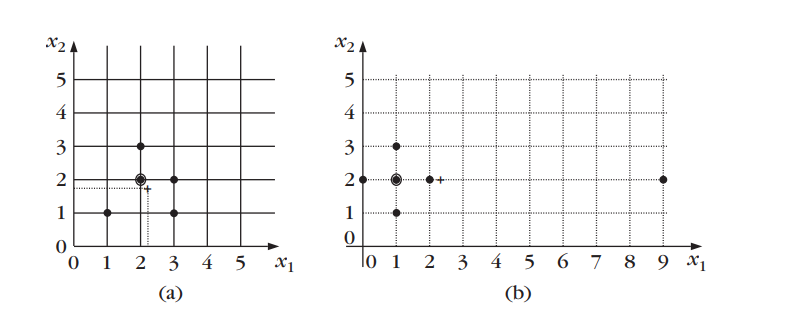
\includegraphics[width=1\linewidth]{2.png}
        \label{fig:enter-label}
    \end{figure}
\end{frame}

% Section: PAM Algorithm
\section{PAM Algorithm}

\begin{frame}{Partitioning Around Medoids (PAM)}
    \begin{itemize}
        \item Used to determine the set of the m medoids that best represent the data set
        \item Iteratively swaps medoids with non-medoids to minimize cost.
        \item Time Complexity: \(O(m(N-m)^2)\).
    \end{itemize}
\end{frame}

\begin{frame}{PAM Algorithm: Optimization Approach}
    \begin{itemize}
        \item PAM minimizes \(J(\mathcal{M}, U)\), where \(\mathcal{M}\) is the set of medoids.
        \item Constraints: Medoids are actual elements from dataset \(X\).
        \item Two sets of medoids \(\mathcal{M}\) and \(\mathcal{M'}\) are \textbf{neighbors} if they share \(m-1\) elements.
        \item A neighbor \(\mathcal{M}_{ij}\) results from replacing \(x_i\) with \(x_j\).
    \end{itemize}
\end{frame}

\begin{frame}{PAM Algorithm: Iterative Improvement}
    \begin{itemize}
        \item Start with a random set \(\mathcal{M}\) of \(m\) medoids.
        \item For each neighbor \(\mathcal{M}_{ij}\), compute:
            \[
            \Delta J_{ij} = J(\mathcal{M}_{ij}, U_{ij}) - J(\mathcal{M}, U)
            \]
        \item If \(\Delta J_{qr} = \min(\Delta J_{ij}) < 0\), replace \(\mathcal{M}\) with \(\mathcal{M}_{qr}\).
        \item Repeat until no further improvement.
    \end{itemize}
\end{frame}

\begin{frame}{Computation of \(\Delta J_{ij}\)}
    \begin{itemize}
        \item \(\Delta J_{ij}\) is computed by summing individual point contributions:
        \[
        \Delta J_{ij} = \sum_{h \in X \setminus \mathcal{M}} C_{hij}
        \]
        \item Four cases determine \(C_{hij}\), depending on:
        \begin{itemize}
            \item Whether \(x_h\) belongs to the cluster of \(x_i\).
            \item Whether \(x_j\) is closer than the second nearest medoid.
        \end{itemize}
    \end{itemize}
\end{frame}

\begin{frame}{Case 1: Retains Second Closest Medoid}
    \begin{itemize}
        \item \(x_h\) belongs to the cluster of \(x_i\).
        \item After replacing \(x_i\) with \(x_j\), \(x_h\) is now represented by the second closest medoid \(x_{h2}\).
        \item The cost change is:
        \[
        C_{hij} = d(x_h, x_{h2}) - d(x_h, x_i) \geq 0
        \]
    \end{itemize}

    \begin{center}
        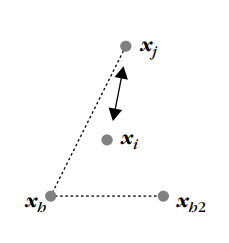
\includegraphics[width=0.35\linewidth]{image.png}
    \end{center}
\end{frame}

\begin{frame}{Case 2: Switches to New Medoid}
    \begin{itemize}
        \item \(x_h\) was initially assigned to \(x_i\).
        \item After replacing \(x_i\) with \(x_j\), \(x_h\) now moves to \(x_j\).
        \item The cost change is:
        \[
        C_{hij} = d(x_h, x_j) - d(x_h, x_i)
        \]
    \end{itemize}
 \begin{center}
        \begin{minipage}{0.45\linewidth}
            \centering
            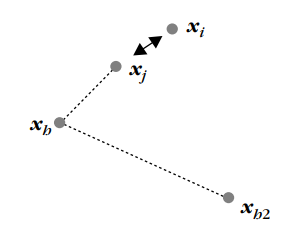
\includegraphics[width=\linewidth]{Case2.png}
        \end{minipage}
        \hfill
        \begin{minipage}{0.45\linewidth}
            \centering
            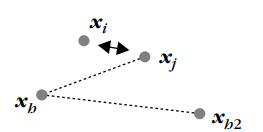
\includegraphics[width=\linewidth]{Case3.png}
        \end{minipage}
    \end{center}
\end{frame}

\begin{frame}{Case 3: Remains in the Same Cluster}
    \begin{itemize}
        \item \(x_h\) is not assigned to \(x_i\), and the replacement does not affect its assignment.
        \item Thus, there is no change in cost:
        \[
        C_{hij} = 0
        \]
    \end{itemize}
    \begin{center}
        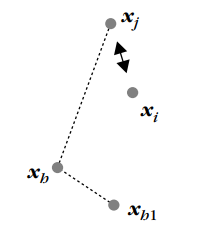
\includegraphics[width=0.3\linewidth]{C4.png}  % Attach your image here
    \end{center}
\end{frame}

\begin{frame}{Case 4: Moves from a Different Medoid}
    \begin{itemize}
        \item \(x_h\) was initially assigned to a different medoid \(x_{h1}\).
        \item After the replacement, \(x_h\) is now assigned to \(x_j\).
        \item The cost change is:
        \[
        C_{hij} = d(x_h, x_j) - d(x_h, x_{h1}) \geq 0
        \]
    \end{itemize}
    \begin{center}
        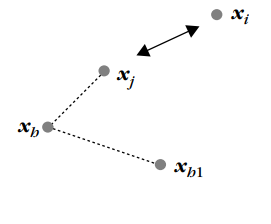
\includegraphics[width=0.5\linewidth]{c5.png}  % Attach your image here
    \end{center}
\end{frame}


% Section: CLARA and CLARANS
\section{CLARA and CLARANS}
\begin{frame}{CLARA and CLARANS}
    \begin{itemize}
        \item \textbf{CLARA}: Draw randomly a sample X'
 of size N' from the entire data set, X and to determine the set of the medoids M' that best represents X' using the PAM algorithm
        \item \textbf{CLARANS}:PAM is applied on the entire data set X, but with a slight modification. At each iteration, not all neighbors of the current set of medoids are considered. Instead, only a randomly selected fraction 
        \[
        q < m(N - m)
        \]
        of them is utilized.
        
    \end{itemize}
\end{frame}
\begin{frame}{CLARA and CLARANS}
    \begin{itemize}
        \item CLARANS is more accurate but computationally expensive.
        \item In some cases CLARA runs significantly faster than CLARANS. It must be pointed out that CLARANS retains its quadratic computational nature and is thus not appropriate for very large data sets.
    \end{itemize}
\end{frame}

% Section: Conclusion
\section{Conclusion}
\begin{frame}{Conclusion}
    \begin{itemize}
        \item \textbf{k-Means}: Simple and efficient but sensitive to initialization.
        \item \textbf{k-Medoids}: More robust but computationally heavier.
        \item \textbf{CLARA and CLARANS}: Trade-off between speed and accuracy.
        \item \textbf{Suggested numbers in CLARA}: Experimental studies suggest that five X' and N' = 40 + 2m lead to satisfactory results.
        \item \textbf{Suggested numbers in CLARANS}: Experimental studies suggest that q can be chosen as the maximum between 0.12m (N - m) and 250.
    \end{itemize}
\end{frame}

\end{document}
